% !TeX root = report.tex
% !TeX encoding = UTF-8
% !TeX spellcheck = en_US
% !TeX document-id = {df60852a-801d-4958-af2e-e2c2af582758}
% !TeX TXS-program:compile = txs:///pdflatex/[--shell-escape]
%
% Report for Boston Housing Prices
% Udacity MLND Project 1
%
% Aravind Battaje

\documentclass{article}
\usepackage[margin=1in]{geometry}
\usepackage{minted}
\usepackage{multirow}
\usepackage{tabularx}
\usepackage{graphicx}
\usepackage{caption}
\usepackage{subcaption}
\begin{document}	
	\newmint[py]{python}{}
	\newminted[pycode]{python}{}
	\newmintinline[pyinl]{python}{}
	\title{Project Report: Predicting Boston Housing Prices}
	\author{Aravind Battaje}
	\maketitle
	\section{Project Steps}
	The project aims to predict housing prices by using regression learning on some known data. On a comprehensive dataset provided by \texttt{scikit-learn}, preliminary statistical analysis is performed to find the nature of data/features. The dataset is split after shuffling into two sets for training and testing. The training set is used with a decision tree learner at varying tree depths. For each depth, training and testing errors as a function of training set size are computed and graphed. Another graph to assess model complexity (depth of decision tree) in relation to training and testing errors is also computed. The relation of training size with errors and the approximate optimal tree depth is observed from the graph plots. Finally, a cross-validated grid search is used to find the optimal decision tree depth. This is used to predict the house price for a user-input data.
	\section{Statistical Analysis and Data Exploration}
	\subsection{Dataset}
	\texttt{scikit-learn}'s Boston housing dataset possesses following characteristics:
	\begin{center}
		\begin{tabularx}{\textwidth}{c | l X}
			\hline
			      \multicolumn{2}{c}{Number of features}       & 13                                                                    \\ \hline
			    \multicolumn{2}{c}{Number of data points}      & 506                                                                   \\ \hline
			\multirow{13}{5cm}{Feature descriptions} & CRIM    & per capita crime rate by town                                         \\
			                                         & ZN      & proportion of residential land zoned for lots over 25,000 sq.ft.      \\
			                                         & INDUS   & proportion of non-retail business acres per town                      \\
			                                         & CHAS    & Charles River dummy variable (= 1 if tract bounds river; 0 otherwise) \\
			                                         & NOX     & nitric oxides concentration (parts per 10 million)                    \\
			                                         & RM      & average number of rooms per dwelling                                  \\
			                                         & AGE     & proportion of owner-occupied units built prior to 1940                \\
			                                         & DIS     & weighted distances to five Boston employment centers                  \\
			                                         & RAD     & index of accessibility to radial highways                             \\
			                                         & TAX     & full-value property-tax rate per \$10,000                             \\
			                                         & PTRATIO & pupil-teacher ratio by town                                           \\
			                                         & B       & $1000(B_k - 0.63)^2$ where $B_k$ is the proportion of blacks by town  \\
			                                         & LSTAT   & \% lower status of the population                                     \\ \hline
			      \multicolumn{2}{c}{Target description}       & median value of owner-occupied homes in \$1000s                       \\ \hline
		\end{tabularx}
	\end{center}
	The above information can be accessed from the \pyinl/.DESCR/ member of Boston dataset object.
	\subsection{Analysed Characteristics}
	From the dataset loaded, the minimum, maximum, mean, median and standard deviation values of each feature including that of target were found using relevant \emph{numpy} methods. Table \ref{tab:datasetAnalysisTable} is derived from the analyzed data. Note for instance from \textbf{TARGET} column that the mean of target house prices is $22.53 (\times \$1000)$.
	\begin{table}[ht]
		\centering
		\begin{tabularx}{\textwidth}{l|XXXXXXXX}
			\hline
			&     CRIM &       ZN &    INDUS &     CHAS &      NOX &       RM &      AGE &      DIS \\
			\hline
			MIN &  0.00632 &   0      &  0.46    & 0        & 0.385    & 3.561    &   2.9    &  1.1296  \\
			MAX & 88.9762  & 100      & 27.74    & 1        & 0.871    & 8.78     & 100      & 12.1265  \\
			AVG &  3.59376 &  11.3636 & 11.1368  & 0.06917  & 0.554695 & 6.28463  &  68.5749 &  3.79504 \\
			MED &  0.25651 &   0      &  9.69    & 0        & 0.538    & 6.2085   &  77.5    &  3.20745 \\
			STD &  8.58828 &  23.2994 &  6.85357 & 0.253743 & 0.115763 & 0.701923 &  28.121  &  2.10363 \\
		\end{tabularx}		
		\begin{tabularx}{\textwidth}{l|XXXXX >{\bfseries}X}
			\hline
			&      RAD &     TAX &   PTRATIO &        B &   LSTAT &   TARGET \\
			\hline
			MIN &  1       & 187     &  12.6     &   0.32   &  1.73   &  5       \\
			MAX & 24       & 711     &  22       & 396.9    & 37.97   & 50       \\
			AVG &  9.54941 & 408.237 &  18.4555  & 356.674  & 12.6531 & 22.5328  \\
			MED &  5       & 330     &  19.05    & 391.44   & 11.36   & 21.2     \\
			STD &  8.69865 & 168.37  &   2.16281 &  91.2046 &  7.134  &  9.18801 \\
			\hline
		\end{tabularx}
		\caption{Boston housing prices dataset analysis}
		\label{tab:datasetAnalysisTable}	
	\end{table}
	\section{Evaluating Model Performance}
	\subsection{Performance Metric}
	\texttt{scikit-learn} provides five different metrics for assessing model performance, namely, \texttt{mean\_squared\_error}, \\ \texttt{mean\_absolute\_error}, \texttt{median\_absolute\_error}, \texttt{explained\_variance\_score} and \texttt{r2\_score}. \texttt{r2\_score} and \texttt{explained\_variance\_score} are \emph{score} metrics (greater the better, unlike \emph{error} metric) and they help to assess how well the (training) data has been fit on the regressor. This property might not fair well against finding score of testing data and might lead to over-fitting. \texttt{mean\_squared\_error, mean\_absolute\_error} and \texttt{median\_absolute\_error} are simpler metrics and they should fair better against over-fitting. Amongst the \emph{error} metrics, \texttt{median\_absolute\_error} and \texttt{mean\_absolute\_error} will give similar error scores, but differ in that the latter is not robust against outliers; \texttt{mean\_squared\_error} too tends to amplify the effect of outliers. The best performance metric to use thus in this project must be \texttt{median\_absolute\_error}. 
	\begin{figure}[!ht]
		\centering
		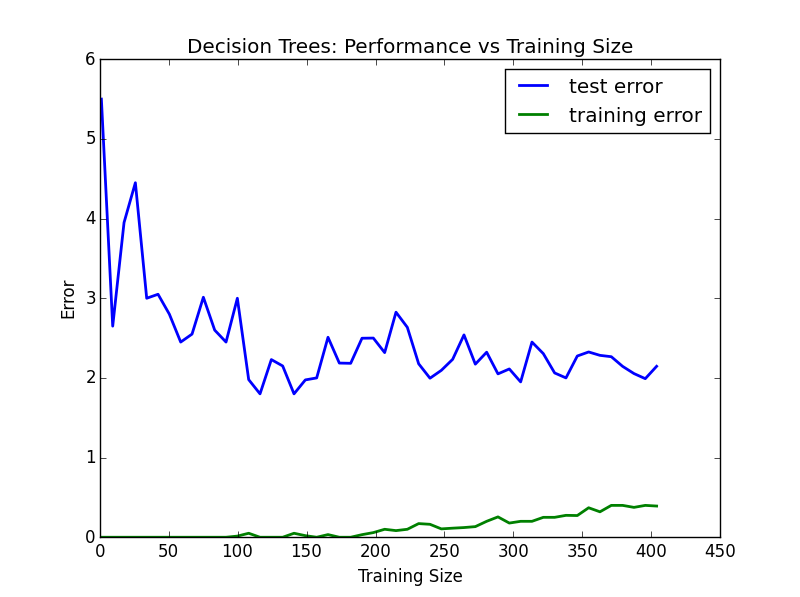
\includegraphics[scale=0.5]{example_decision_tree_error_graph_depth_9}
		\caption{Decision tree of max. depth = 9}
		\label{fig:decisionTreeDepth9}
	\end{figure}
	\subsection{Dataset Split}	 
	The Boston housing data is split into two sets for training and testing purposes. The training set is used during the learning/fitting and the testing set is used to find the (true) prediction deviation from target values. If there is no split in data, and the learner is modeled only on the given dataset, the chances of over-fitting is high. Effectively, by splitting the data and performing the test step, it is ensured that the model is generalized on the data. The over-fitting for instance is observable in Figure \ref{fig:decisionTreeDepth9}, where predicting on training set, which is when the regressor hasn't seen any \emph{new} (or test) data, the training error is very low for any training size. Also, the ratio of split plays a role in model performance. If the training data size is lower than test data size, \emph{optimum} learning might not be possible. It is also bad to have a very small test data size as that might lead to over-fitting. For the project, optimum \texttt{TrainSize:TestSize} ratio could be between $50\%$ to $80\%$.
	\subsection{Grid Search and Cross-Validation}
	\texttt{scikit-learn}'s \pyinl/GridSearchCV/ helps perform an exhaustive grid search on the \emph{parameter grid} of an \emph{estimator}. In the project, a regression based \emph{estimator} (\pyinl/DecisionTreeRegressor/) is used. \pyinl/DecisionTreeRegressor/ has a parameter called \pyinl/maxdepth/ that controls the maximum allowed tree depth. Given a parameter space, grid search exhaustively evaluates the \emph{estimator} performance for each parameter (here only \pyinl/maxdepth/). This helps to find the best model to fit the data. 
	\paragraph{}Additionally, \pyinl/GridSearchCV/ uses cross-validation instead of train-test split to learn and evaluate the model performance. Cross-validation is a procedure where the input dataset is split into smaller chunks, followed by learning on most of the chunks, holding out only a few for evaluation. In the most basic form (used here), called \emph{K-Fold} cross-validation, data is split into $K$ \emph{folds}. $K-1$ folds are used for learning and the left out fold is used to evaluate model performance. With several iterations, the fold held out is made to cycle through all available $K$ folds. The total performance measure will be the average of performace metric calculated in each iteration. In the project, a \emph{3-Fold} (default) cross-validated grid search is used, which is also optimum. Higher folds might result in smaller validation set, effectively over-fitting. Anything more than \emph{10-Fold} cross-validation with Boston housing dataset might not be prudent because of the small size of data (506).
	\section{Analyzing Model Performance}
	\subsection{Learning Curves}
	\begin{figure}[h]
		\centering
		\begin{subfigure}[b]{0.4\textwidth}
			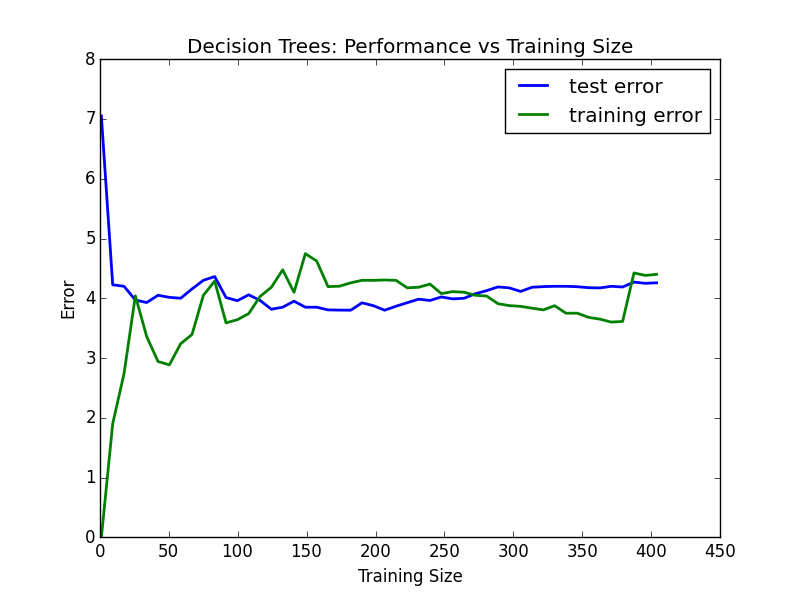
\includegraphics[width=\textwidth]{decision_tree_error_graph_depth_1}
			\caption{Depth 1}
			\label{fig:decisionTreeDepth1}
		\end{subfigure}
		\begin{subfigure}[b]{0.4\textwidth}
			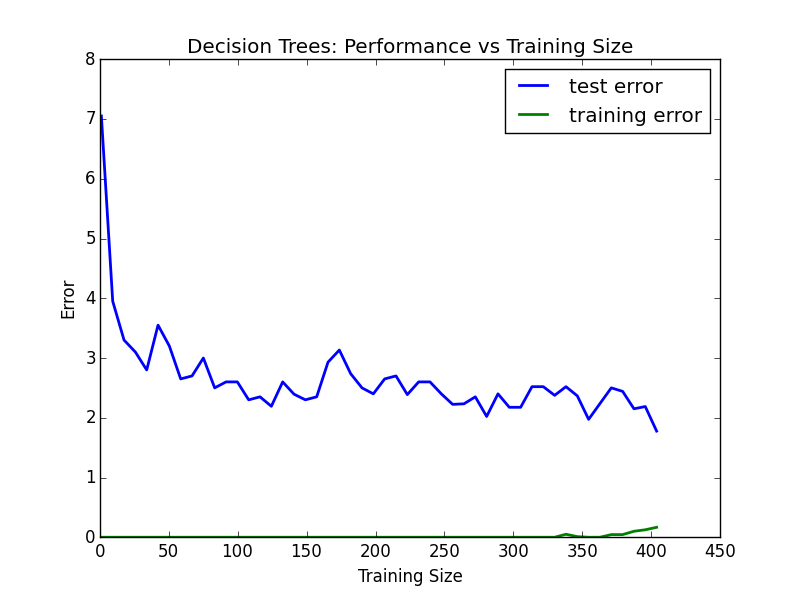
\includegraphics[width=\textwidth]{decision_tree_error_graph_depth_10}
			\caption{Depth 10}
			\label{fig:decisionTreeDepth10}
		\end{subfigure}
		\caption{Decision tree learning curves}
	\end{figure}
	In the project, ten training curves are generated with ten different \emph{max depths}. In each of the graphs, the training and testing errors as a function of training size (50 increments) is plotted. The ten plots give an insight into the nature of \emph{learning} with respect to the training size and model complexity (max depth). Figure \ref{fig:decisionTreeDepth1} (max depth 1) and Figure \ref{fig:decisionTreeDepth10} (max depth 10) represent the extremes in this series of plots . In Figure \ref{fig:decisionTreeDepth1}, it is quite apparent that the \emph{learning} by the decision tree is insufficient because training and testing errors are quite high and they converge as the training size increases. On the other hand, Figure \ref{fig:decisionTreeDepth10} represents another extreme where with sufficient training sizes, testing error decreases, but more importantly, the training error is very close to zero. This indicates that the decision tree has fit the training data quite well (maybe  too well, or over-fit). 
	\paragraph{}In general for both plots, it can be seen that rising training data size and rising max depths, result in lesser error with testing data. The curve is quite abrupt in Figure \ref{fig:decisionTreeDepth1} because of the terrible under-fitting. The training errors in both plots is very low when the training size is too low as a consequence of over-fitting on the very small size of data.
	\subsection{Model Complexity}
	\begin{figure}[h]
		\centering
		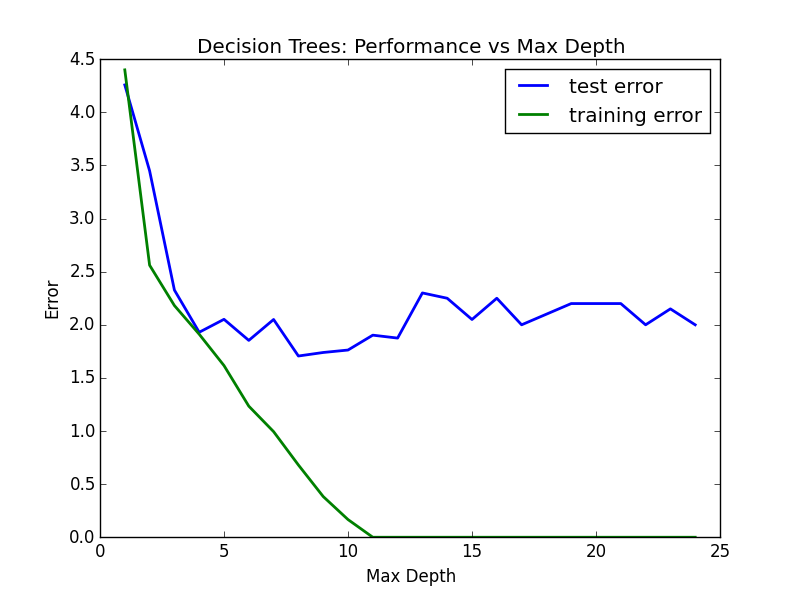
\includegraphics[scale=0.4]{model_complexity_graph}
		\caption{Model complexity graph}
		\label{fig:modelComplexity}
	\end{figure}
	The model complexity graph (Figure \ref{fig:modelComplexity}) represents the relation between learning errors and complexity of the decision tree (or max depth). The same data for training and testing as used for the above mentioned learning curves are used here. Upto a certain point (max depth = 10) each learning curves' training and testing errors at a particular (highest) training size relate to each error point in the model complexity graph. Therefore, as it is observed in learning curves, model complexity graph confirms the fact that the training error decreases and tends to zero with higher max depths as a consequence of over-fitting, and that with higher max depths the testing error seems to decrease. However, it is important to note in the model complexity graph that the testing error seems to saturate beyond a certain max depth. More precisely, the testing error tends to stay around a neighborhood of a minimum, beyond a certain \emph{point} (of generalization). The slight increases in testing error beyond this \emph{point} can be attributed to over-fitting. This could also indicate that with any given set of training data, it is not prudent to achieve a perfect fit without trading off on generalization. Thus, in Figure \ref{fig:modelComplexity}, as the saturation of testing error starts at around a max depth of 5, and training error starts to get too low beyond max depth of 7, the optimum model to select for generalization would be a decision tree of max depth between 5 and 7.
	\section{Model Prediction}
	After running 100 trials, the most common model was found to be a decision tree of max depth 6. The prediction of this tree for the sample input \texttt{[11.95, 0.00, 18.100, 0, 0.6590, 5.6090, 90.00, 1.385, 24, 680.0, 20.20, 332.09, 12.13]} is \texttt{20.76598639}. The average of the predictions, with max depth mostly varying between 5 to 7, was found to be \texttt{20.71604903} with a standard deviation of \texttt{0.33793076}. It appears that the most common prediction \texttt{20.76598639} approximately agrees with the statistics previously derived. For instance, comparing some  of the features of the sample input, such as \texttt{PTRATIO} and \texttt{RM}, against those of statististics, the prediction appears to be consistent. In other words, considering \texttt{PTRATIO} (pupil-teacher ratio) and \texttt{RM} (average number of rooms per dwelling), which have the least variance among the dataset, and are also slightly lesser than the respective means, it appears natural that the prediction also should be lesser than the average. By this logic, the prediction falls well within the \emph{majority of distribution} of housing prices in the dataset.
\end{document}